%%%%%%%%%%%%%%%%%%%%%%%%%%%%%%%%%%%%%%%%%%%%%%%%%%%%%%%%%%%%%%%%%
\documentclass[hyperref={pdfpagelabels=false},compress,table]{beamer} % 在Mac下无法编译
% \documentclass[compress,table]{beamer} % 在Mac下使用
% package for font
\usepackage{fontspec}
\defaultfontfeatures{Mapping=tex-text}  %%如果没有它,会有一些 tex 特殊字符无法正常使用,比如连字符。
\usepackage{xunicode,xltxtra}
\usepackage[BoldFont,SlantFont,CJKnumber,CJKchecksingle]{xeCJK}  % \CJKnumber{12345}: 一万二千三百四十五
\usepackage{CJKfntef}  %%实现对汉字加点、下划线等。
\usepackage{pifont}  % \ding{}
% package for math
\usepackage{amsfonts}

% package for graphics
\usepackage[americaninductors,europeanresistors]{circuitikz}
\usepackage{tikz}
\usetikzlibrary{plotmarks}  % placements=positioning
\usepackage{graphicx}  % \includegraphics[]{}
\usepackage{subfigure}  %%图形或表格并排排列
% package for table
\usepackage{colortbl,dcolumn}  %% 彩色表格
\usepackage{multirow}
\usepackage{multicol}
\usepackage{booktabs}
% package for code
\usepackage{fancyvrb}
\usepackage{listings}

% \usepackage{animate}
% \usepackage{movie15}

%%%%%
% setting for beamer
\usetheme{default} % Madrid(常用), Copenhagen, AnnArbor, boxes(白色), Frankfurt,Berkeley,default
 \useoutertheme[subsection=true]{miniframes} % 使用Berkeley时注释本行
\usecolortheme{sidebartab}
\usefonttheme{serif}  %%英文使用衬线字体
% \setbeamertemplate{background canvas}[vertical
% shading][bottom=white,top=structure.fg!7] %%背景色,上25%的蓝,过渡到下白。
\setbeamertemplate{theorems}[numbered]
\setbeamertemplate{navigation symbols}{}  %% 去掉页面下方默认的导航条
\setbeamercovered{transparent}  %设置 beamer 覆盖效果

% 设置标题title背景色
% \setbeamercolor{title}{fg=black, bg=lightgray!60!white}
\setbeamercolor{title}{fg=white, bg=black!90!white}

% 设置每页小LOGO
\pgfdeclareimage[width=1cm]{ouc}{figures/static/ouc.pdf}
\logo{\pgfuseimage{ouc}{\vspace{-20pt}}}

% setting for font
%%\setCJKmainfont{Adobe Kaiti Std}
\setCJKmainfont{SimSun} 
%% \setCJKmainfont{FangSong_GB2312} 
%% \setmainfont{Apple Garamond}  %%苹果字体没有SmallCaps
\setmainfont{Times New Roman}
%FUNNY%\setCJKmainfont{DFPShaoNvW5-GB}  %%华康少女文字W5(P)
%FUNNY%\setCJKmainfont{FZJingLeiS-R-GB}  %%方正静蕾体
%FUNNY%\setmainfont{Purisa}
%\setsansfont[Mapping=tex-text]{Adobe Song Std}
     %如果装了Adobe Acrobat,可在font.conf中配置Adobe字体的路径以使用其中文字体。
     %也可直接使用系统中的中文字体如SimSun、SimHei、微软雅黑等。
     %原来beamer用的字体是sans family;注意Mapping的大小写,不能写错。
     %设置字体时也可以直接用字体名,以下三种方式等同:
     %\setromanfont[BoldFont={黑体}]{宋体}
     %\setromanfont[BoldFont={SimHei}]{SimSun}
     %\setromanfont[BoldFont={"[simhei.ttf]"}]{"[simsun.ttc]"}
% setting for graphics
\graphicspath{{figures/}}  %%图片路径
\renewcommand\figurename{图}

% setting for pdf
\hypersetup{% pdfpagemode=FullScreen,%
            pdfauthor={Xiaodong Wang},%
            pdftitle={Title},%
            CJKbookmarks=true,%
            bookmarksnumbered=true,%
            bookmarksopen=false,%
            plainpages=false,%
            colorlinks=true,%
            citecolor=green,%
            filecolor=magenta,%
            linkcolor=blue,%red(default)
            urlcolor=cyan}

% setting for fontspec
\XeTeXlinebreaklocale "zh"  %%表示用中文的断行
\XeTeXlinebreakskip = 0pt plus 1pt minus 0.1pt  %%多一点调整的空间
%%%%%

% 设置文字版式为两端对齐
\renewcommand{\raggedright}{\leftskip=0pt \rightskip=0pt plus 0cm}
\raggedright 

% font setting by xeCJK
\setCJKfamilyfont{NSimSun}{NSimSun}
\newcommand{\song}{\CJKfamily{NSimSun}}
%%%\setCJKfamilyfont{AdobeSongStd}{Adobe Song Std}
%%%\newcommand{\AdobeSong}{\CJKfamily{AdobeSongStd}}
\setCJKfamilyfont{FangSong}{FangSong_GB2312}
\newcommand{\fang}{\CJKfamily{FangSong}}
%%%\setCJKfamilyfont{AdobeFangsongStd}{Adobe Fangsong Std}
%%%\newcommand{\AdobeFang}{\CJKfamily{AdobeFangsongStd}}
\setCJKfamilyfont{SimHei}{SimHei}
\newcommand{\hei}{\CJKfamily{SimHei}}
%%%\setCJKfamilyfont{AdobeHeitiStd}{Adobe Heiti Std}
%%%\newcommand{\AdobeHei}{\CJKfamily{AdobeHeitiStd}}
\setCJKfamilyfont{KaiTi}{KaiTi}
\newcommand{\kai}{\CJKfamily{KaiTi}}
%%%\setCJKfamilyfont{AdobeKaitiStd}{Adobe Kaiti Std}
\newcommand{\AdobeKai}{\CJKfamily{AdobeKaitiStd}}
\setCJKfamilyfont{LiSu}{LiSu}
\newcommand{\li}{\CJKfamily{LiSu}}
\setCJKfamilyfont{YouYuan}{YouYuan}
\newcommand{\you}{\CJKfamily{YouYuan}}
\setCJKfamilyfont{FZJingLei}{FZJingLeiS-R-GB}
\newcommand{\jinglei}{\CJKfamily{FZJingLei}}
\setCJKfamilyfont{MSYH}{Microsoft YaHei}
\newcommand{\msyh}{\CJKfamily{MSYH}}

% 自定义颜色
\def\Red{\color{red}}
\def\Green{\color{green}}
\def\Blue{\color{blue}}
\def\Mage{\color{magenta}}
\def\Cyan{\color{cyan}}
\def\Brown{\color{brown}}
\def\White{\color{white}}
\def\Black{\color{black}}

\lstnewenvironment{javaCode}[1][]{% for Java
  \lstset{
    basicstyle=\tiny\ttfamily,%
    columns=flexible,%
    framexleftmargin=.7mm, %
    frame=shadowbox,%
    rulesepcolor=\color{cyan},%
    % frame=single,%
    backgroundcolor=\color{white},%
    xleftmargin=2\fboxsep,%
    xrightmargin=2\fboxsep,%
    %numbers=left,numberstyle=\tiny,%
    numberblanklines=false,numbersep=7pt,%
    language=Java, %
    }\lstset{#1}}{}

\lstnewenvironment{xmlCode}[1][]{% for Java
  \lstset{
    basicstyle=\tiny\ttfamily,%
    columns=flexible,%
    framexleftmargin=.7mm, %
    frame=shadowbox,%
    rulesepcolor=\color{cyan},%
    % frame=single,%
    backgroundcolor=\color{white},%
    xleftmargin=2\fboxsep,%
    xrightmargin=2\fboxsep,%
    %numbers=left,numberstyle=\tiny,%
    numberblanklines=false,numbersep=7pt,%
    language=html, %
    }\lstset{#1}}{}

\lstnewenvironment{shCode}[1][]{% for Java
  \lstset{
    basicstyle=\scriptsize\ttfamily,%
    columns=flexible,%
    framexleftmargin=.7mm, %
    frame=shadowbox,%
    rulesepcolor=\color{brown},%
    % frame=single,%
    backgroundcolor=\color{white},%
    xleftmargin=4\fboxsep,%
    xrightmargin=4\fboxsep,%
    numbers=left,numberstyle=\tiny,%
    numberblanklines=false,numbersep=7pt,%
    language=sh, %
    }\lstset{#1}}{}

\newcommand\ask[1]{\vskip 4bp \tikz \node[rectangle,rounded corners,minimum size=6mm,
  fill=white,]{\Cyan \includegraphics[height=1.5cm]{question} \Large \msyh #1};}

\newcommand\wxd[1]{\vskip 4bp \tikz \node[rectangle,minimum size=6mm,
  fill=blue!60!white,]{\White \ding{118} \msyh #1};}

\newcommand\xyy[1]{\vskip 2bp \tikz \node[rectangle,minimum size=3mm,
  fill=black!80!white,]{\White \msyh\scriptsize #1};}

\newcommand\cxf[1]{\vskip 4bp \tikz \node[rectangle,rounded corners,minimum size=6mm,
  fill=orange!60!white,]{\White \ding{42} \msyh #1};}

\newcommand\samp[1]{\vskip 2bp \tikz \node[rectangle,minimum size=3mm,
  fill=white!100!white,]{\Mage\msyh \small CODE \ding{231} \Black #1};\vskip -8bp}

\newcommand\zhyfly[1]{\tikz \node[rectangle,rounded corners,minimum size=6mm,ball
  color=red!25!blue,text=white,]{#1};}

\newcommand\pno[1]{\tikz \node[rectangle,rounded corners,minimum size=1mm,
  fill=yellow!50!black,text=white,]{\msyh\scriptsize P. #1};}

\setbeamerfont{frametitle}{series=\msyh} % 修改Beamer标题字体

\makeatletter
\newcommand{\Extend}[5]{\ext@arrow 0099{\arrowfill@#1#2#3}{#4}{#5}}
\makeatother

%%%%%%%%%%%%%%%%%%%%%%%%%%%%%%%%%%%%%%%%%%%%%%%%%%%%%%%%%%%%%%%%% 
% \titlepage
\title[KevinW@OUC]{\hei {\Large 基于Java EE的企业应用系统设计\\Spring MVC}}
\author[王晓东]{王晓东\\
  \href{mailto:wangxiaodong@ouc.edu.cn}{\footnotesize wangxiaodong@ouc.edu.cn}}
\institute[中国海洋大学]{\small 中国海洋大学}
\date{\today}
\titlegraphic{\vspace{-6em}
\includegraphics[height=6cm]{static/ouc.pdf}\vspace{-6em}}

%%%%% 
\begin{document}
%% Delete this, if you do not want the table of contents to pop up at
%% the beginning of each subsection:
\AtBeginSection[]{                              % 在每个Section前都会加入的Frame
  \frame<handout:0>{
    \frametitle{\textbf{\hei 接下来…}}
    \tableofcontents[currentsection]
  }
}  %

\AtBeginSubsection[]                            % 在每个子段落之前
{
  \frame<handout:0>                             % handout:0 表示只在手稿中出现
  {
    \frametitle{\textit{\hei 接下来…}}\small
    \tableofcontents[current,currentsubsection] % 显示在目录中加亮的当前章节
  }
}
 \frame{\titlepage}

%%%%%%%%%%%%%%%%%%%%%%%%%%%%%%%%%%%%%%%%%%%%%%%%
\begin{frame}
\frametitle{References}
\begin{enumerate}
\item Spring MVC: A Tutorial (Second Edition) (ISBN 9781771970310)
\end{enumerate}  
\end{frame}

% \begin{frame}
% \frametitle{本章学习目标}
% \begin{enumerate}
% \item 
% \end{enumerate}  
% \end{frame}

\section*{大纲}
\frame{\frametitle{大纲} \tableofcontents }

%%%%%%%%%%%%%%%%%%%%%%%%%%%%%%%%%%%%%%%%%%%%%%%%%%
\section{Java Web应用的开发演化}

\begin{frame}[fragile] % [fragile]参数使得能够插入代码
\frametitle{JSP方式}

JSP在HTML代码里写Java代码完成业务逻辑。

\begin{xmlCode}
<%
     String name = request.getParameter("name");
     String password = request.getParameter("password");

     UserHandler userHandler = new UserHandler();
     if(userHandler.authenticate(name, password)) {
%>
<p>Congratulations, login successfully. </p>
<%
      } else {
%>
<p>Sorry, login failed.</p>
<%
      }
%>
\end{xmlCode}
\end{frame}

\begin{frame}[fragile] % [fragile]参数使得能够插入代码
\frametitle{JSP方式}

\wxd{仅有的一点优势}\kai
\begin{enumerate}
\item 无需额外的配置文件,无需框架的帮助,即可完成逻辑。
\item 简单易上手。
\end{enumerate}

\wxd{劣势}
\begin{enumerate}[<+-| alert@+>]\kai
\item Java代码由于混杂在一个HTML环境中而显得混乱不堪,可读性非常差。一
  个JSP文件有时候会变成几十K,甚至上百K,经常难以定位逻辑代码的所在。
\item 编写代码时非常困惑,不知道代码到底应该写在哪里,也不知道别人是不
  是已经曾经实现过类似的功能,到哪里去引用。
\item 突然之间,某个需求发生了变化。于是,每个人蒙头开始全程替换,还要
  小心翼翼的,生怕把别人的逻辑改了。
\item 逻辑处理程序需要自己来维护生命周期,对于类似数据库事务、日志等众
  多模块无法统一支持。
\end{enumerate}
\end{frame}

\begin{frame}[fragile] % [fragile]参数使得能够插入代码
\frametitle{需求的变化}

如果有一种方式能够将页面上的那些Java代码抽取出来,让页面上尽量少出现Java代码该有多好!

{\Blue\hei 于是许多人开始使用servlet来处理那些业务逻辑。 }

\end{frame}

\begin{frame}[fragile] % [fragile]参数使得能够插入代码
\frametitle{Servlet方式}

\begin{javaCode}
public class LoginServlet extends HttpServlet {
  
  @Override
  protected void doPost(HttpServletRequest req,
  HttpServletResponse resp) throws ServletException, IOException {
    String message = null;
    RequestDispatcher dispatcher = req.
      getRequestDispatcher("/result.jsp");
    String name = req.getParameter("name");
    String password = req.getParameter("password");
    
    UserHandler userHandler = new UserHandler();
    if(userHandler.authenticate(name, password)) {
      message = "恭喜你,登录成功";
    } else {
      message = "对不起,登录失败";
    }
    
    req.setAttribute("message", message);
    dispatcher.forward(req, resp);
  }
}
\end{javaCode}
\end{frame}

\begin{frame}[fragile] % [fragile]参数使得能够插入代码
\frametitle{Servlet方式}

同时,我们需要在web.xml中为这个servlet配置url的请求映射关系。 

\begin{xmlCode}
<servlet>
  <servlet-name>Login</servlet-name>
  <servlet-class>com.demo2do.servlet.LoginServlet</servlet-class>
</servlet>

<servlet-mapping>
  <servlet-name>Login</servlet-name>
  <url-pattern>/Login</url-pattern>
</servlet-mapping>
\end{xmlCode}
\end{frame}

\begin{frame}[fragile] % [fragile]参数使得能够插入代码
\frametitle{框架方式}

时代进一步发展,人们发现简单的JSP和Servlet已经很难满足人们懒惰的要求了。
于是,人们开始试图总结一些公用的Java类,来解决Web开发过程中碰到的问题。
如Struts、Spring MVC,它们非常先进地实现了{\hei\Red MVC模式}。
\end{frame}

\begin{frame}[fragile] % [fragile]参数使得能够插入代码
\frametitle{那么我们需要什么?}

在回顾写代码的历史之后,回头来看我们到底需要什么? 

无论是使用JSP,还是使用Struts,或是Spring MVC,我们至少都需要一些必须的
元素:

\begin{enumerate}[<+-| alert@+>]
\item {\hei 数据 }\only<1>{在这个例子中,就是name和password。他们共同构成了程序数据的核心
    载体。事实上,我们往往会有一个User类来封装name和password,这样会使得我们的程序更加OO。
    无论怎么说,数据会穿插在这个程序的各处,成为程序运行的核心。 }
\item {\hei 页面展示 }\only<2>{在这个例子中,就是login.jsp。没有这个页面,一切的请求、验
    证和错误展示也无从谈起。在页面上,我们需要利用HTML,把我们需要展现的数据都呈现出来。
    同时我们也需要完成一定的页面逻辑,例如,错误展示,分支判断等。 }
\item {\hei 处理具体业务的场所 }\only<3>{不同阶段,处理具体业务的场所就不太一样。原来
      用JSP和Servlet,后来用Struts的Action、Spring的Controller。 }
\end{enumerate}
\end{frame}

\begin{frame}[fragile] % [fragile]参数使得能够插入代码
\frametitle{MVC}

上面的这些必须出现的元素,在不同的时代被赋予了不同的表现形式,有的受到时代的束缚,其表现
形式非常落后,有的已经不再使用。但是拨开这些外在的表现形式,我们就可以发现,这就是我们已
经熟悉的MVC。

\begin{itemize}
\item 数据 \ding{235} Model 
\item 页面展示 \ding{235} View 
\item 处理具体业务的场所 \ding{235} Control
\end{itemize}

{\Red\hei 框架不重要。只要能够深刻理解MVC的概念,框架只是几个jar包而已。}
\end{frame}

\begin{frame}[fragile] % [fragile]参数使得能够插入代码
\frametitle{MVC}

\begin{figure}
\centering
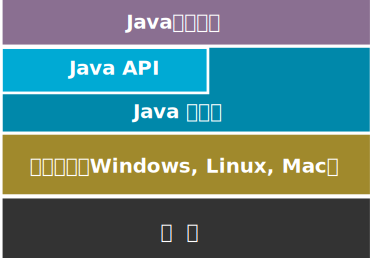
\includegraphics[width=0.9\textwidth]{fig02.pdf}
\end{figure}
\end{frame}

\begin{frame}[fragile] % [fragile]参数使得能够插入代码
\frametitle{MVC的特点}\kai
\begin{enumerate}
\item 多个视图可以对应一个模型,可以减少代码的复制,在模型发生改变时,易于维护。
\item 模型返回的数据与显示逻辑分离。模型数据可以应用任何显示技术,例如,使用JSP、Velocity模板或者直接产生Excel。
\item 应用被分为三层,降低各层耦合,提高了可扩展性。
\item 控制层把不同模型和视图组合在一起,完成不同的请求,控制层包含了用户请求权限的概念。
\item MVC符合软件工程化管理的思想,不同层各司其职,有利于通过工程化和工具化产生管理程序代码。
\end{enumerate}
\end{frame}

\begin{frame}[fragile] % [fragile]参数使得能够插入代码
\frametitle{MVC}

数据是动的,数据在View和Control层一旦运动起来,就会产生许多的问题:

\begin{itemize}[<+-| alert@+>]\kai\small
\item 数据从View层传递到Control层,如何使得一个个扁平的字符串,转化成一
  个个生龙活虎的Java对象。
\item 数据从View层传递到Control层,如何方便的进行数据格式和内容的校验? 
\item 数据从Control层传递到View层,一个个Java对象,又如何在页面上以各种
  各样的形式展现出来。
\item 如果试图将数据请求从View层发送到Control层,你如何才能知道你要调用
  的究竟是哪个类,哪个方法?一个Http的请求,又如何与Control层的Java代码
  建立起关系来?
\end{itemize}
\end{frame}

\begin{frame}[fragile] % [fragile]参数使得能够插入代码
\frametitle{框架}

框架是为了解决一个又一个在Web开发中所遇到的问题而诞生的。不同的框架,都
是为了解决不同的问题,但是对于程序员而言,他们仅仅是jar包而已。框架的优
缺点的评论,也完全取决于其对问题解决程度和解决方式的优雅性的评论。所
以,{\hei\Blue 千万不要为了学习框架而学习框架,而是要为了解决问题而学习
  框架!}
\end{frame}

\section{MVC模式示例}

\begin{frame}[fragile]
  \frametitle{应用功能说明}

  应用功能设定为输入一个产品信息并展示,流程为:

  \begin{itemize}
  \item 用户填写产品表单并提交;
  \item 应用保存产品并展示一个完成页面,显示己保存的产品信息。
  \end{itemize}
  
\end{frame}

\begin{frame}[fragile]
  \frametitle{程序设计}

  \wxd{应用支持以下两个Action}
  
  \begin{itemize}\kai
  \item 发送输入表单到浏览器上,展示“添加产品”表单,其对应的URI应包含字符串product\_input;
  \item 保存产品并返回完成页面,对应的URI包含字符串product\_save。
  \end{itemize}  

  \wxd{应用所包含的组件构成}

  \begin{itemize}\kai
  \item 一个Product类,作为product的领域对象;
  \item 一个ProductForm类,封装了HTML表单的输入项;
  \item 一个ControllerServlet类,本示例应用的控制器;
  \item 一个SaveProductAction类;
  \item 两个JSP视图页面(ProductForm.jsp和ProductDetail.jsp);
  \item 一个CSS文件,定义了两个JSP页面的显示风格。
  \end{itemize}
  
\end{frame}

\section{Spring MVC}

\begin{frame}[fragile]
  \frametitle{采用Spring MVC框架开发Web应用的优势}
  
  \wxd{Spring MVC具备的能加速开发的功能列表}
  
  \begin{enumerate}\small
  \item Spring MVC是Spring框架的一部分,可以利用Spring提供的其他能力。
  \item Spring MVC中提供了Dispatcher Servlet而无需额外开发。
  \item Spring MVC中使用基于XML的配置文件,可以编辑配置而无需重新编译应用程序。
  \item Spring MVC实例化控制器,并根据用户输入来构造bean。
  \item Spring MVC可以自动绑定用户输入并正确地转换数据类型。
  \item Spring MVC内置了常见的校验器,可以校验用户输入,若校验不通过则重定向回输入表单。
  \item Spring MVC支持国际化和本地化,支持根据用户区域显示多国语言。
  \item Spring MVC支持多种视图技术,包括JSP技术、Velocity和FreeMarker等。
  \end{enumerate}

\end{frame}

\begin{frame}[fragile]
  \frametitle{Spring MVC的DispatcherServlet}

  Spring MVC自带了一个开箱即用的DispatcherServlet,要使用这个servlet需要在部署描述符web.xml中配置。
  
  \xyy{org.springfamework.web.servlet.DispatcherServlet}

  \begin{xmlCode}
  <servlet>
    <servlet-name>springmvc</servlet-name>
    <servlet-class>
      org.springframework.web.servlet.DispatcherServlet
    </servlet-class>
    <load-on-startup>l</load-on-startup>
  </servlet>
    
  <servlet-mapping>
    <servlet-name>springmvc</servlet-name>
    <!-- Map all requests to the DispatcherServlet -->
    <url-pattern>/</url-pattern>
  </servlet-mapping>
  \end{xmlCode}

  {\Red\small\kai servlet元素内的load-on-startup元素可选。如果它存在,则在
    应用程序启动时装载servlet并调用它的init方法;若不存在,则在
    该servlet的第一个请求到来时加载。}

\end{frame}

\begin{frame}[fragile]
  \frametitle{Spring MVC的DispatcherServlet}

  \wxd{DispatcherServlet的默认配置文件}

  DispatcherServlet会使用Spring MVC诸多默认组件。初始化时会寻找在应用程
  序的WEB-INF目录下的配置文件,该配置文件的命名规则为: {\bf\Red
    servletName-servlet.xml}。

  {\kai 其中,servletName是在部署描述符中的DispatcherServlet的名称。}

  \wxd{指定任意位置的DispatcherServlet配置文件}

  \begin{xmlCode}
  <servlet>
    <servlet-name>springmvc</servlet-name>
    <servlet-class>
      org.springframework.web.servlet.DispatcherServlet
    </servlet-class>
    <init-param>
      <param-name>contextConfigLocation</param-name>
      <param-value>/WEB-INF/confiq/simple-config.xml</param-value>
    </init-param〉
    <load-on-startup>l</load-on-startup>
  </servlet>
  \end{xmlCode}  

\end{frame}

\begin{frame}[fragile]
  \frametitle{Controller}

  \wxd{实现Controller的方法}

  \begin{itemize}
  \item 实现org.springframework.web.servlet.mvc.Controller接口开发控制器,这个接口包含handleRequest方法:

    \begin{javaCode}
    ModelAndView handleRequest(HttpServletRequest request,
      HttpServletResponse response);
    \end{javaCode}

    {\kai\small\Blue 其实现类可以访问对应请求
      的HttpServletRequest和HttpServletResponse对象,还必须返回一个包含
      视图路径或视图模型的ModelAndView对象。Controller接口的实现类只能
      处理一个单一动作。}
    
  \item 基于注解的控制器可以同时支持多个请求处理动作处理,并且无须实现任何接口。
  \end{itemize}
\end{frame}

\begin{frame}[fragile]
  \frametitle{Spring MVC示例}

  \cxf{References: springmvc-intro-01}

\end{frame}

\begin{frame}[fragile]
  \frametitle{View Resolver}

  Spring MVC中的视图解析器负责解析视图,可以通过在配置文件中定义一个ViewResolver来配置视图解析器。

  \begin{xmlCode}
  <bean id="viewResolver" class="org.springframework.web.servlet.
  view.InternalResourceViewResolver">
    <property name="prefix" value="/WEB-INF/jsp/" />
    <property name="suffix" value=".jsp" />
  </bean>
  \end{xmlCode}

  {\Red\kai 视图解析器配置有前缀和后缀两个属性,View路径将缩短。例如,
    仅需提供“myPage”,而不必再设置视图路径为/WEB-INF/jsp/myPage.jsp,
    视图解析器将会自动增加前缀和后缀。}
\end{frame}

\begin{frame}[fragile]
  \frametitle{基于注解的控制器}

  \wxd{使用基于注解的控制器的几个优点}

  \begin{enumerate}
  \item Controller和RequestMapping注释类型是Spring MVC API最重要的两个注释类型。
  \item 一个控制器类可以处理多个动作(而一个实现了Controller接口的控制器只能处理一个动作) 。
  \item 基于注解的控制器的请求映射不需要存储在配置文件中。使用RequestMapping注释类型,可以对一个方法进行请求处理。
  \end{enumerate}

\end{frame}

\begin{frame}[fragile]
  \frametitle{Controller注解类型}

  \xyy{org.springframework.stereotype.Controller} 注解类型用于指示Spring类的实例是一个控制器。

  \wxd{@Controller示例}

  \begin{javaCode}
  package com.example.controller;
  import org.springframework.stereotype.Controller;
  ...
  
  @Controller
  public class CustomerController {
    // request-handling methods here
  }
  \end{javaCode}

\end{frame}

\begin{frame}[fragile]
  \frametitle{Controller注解类型}

  Spring使用扫描机制找到应用程序中所有基于注解的控制器类。为了确
  保Spring能找到控制器,需要在Spring MVC的配置文件中完成以下配置:

  \xyy{声明springcontext}
  \begin{xmlCode}
  <beans
  xmlns:context="http://www.springfrarnework.org/schema/context">
  \end{xmlCode}

  \xyy{应用<component-scan>元素指定控制器类的基本包}
  \begin{xmlCode}
  <context:component-scan base-package="basePackage" />
  \end{xmlCode}

  {\Red\kai 例如,若所有的控制器类都在com.example.controller及
    其子包下,则需要写一个如下所示的<component-scan>元素:}
  \begin{xmlCode}
  <context:component-scan base-package="com.example.controller" />
  \end{xmlCode}
\end{frame}

\begin{frame}[fragile]
  \frametitle{RequestMapping注解类型}

  \xyy{org.springframework.web.bind.annotation.RequestMapping} 在控制类
  的内部为每一个动作开发相应的处理方法,要让Spring知道用哪一种方法来处
  理它的动作,需要使用该注解类型映射URI与方法。
  
  采用@RequestMapping注解的方法将成为请求处理方法,并由调度程序在接收到
  对应URL请求时调用。

  \wxd{@RequestMapping示例}

  \begin{javaCode}
  package com.example.controller;
  import org.springframework.stereotype.Controller;
  import org.springframework.web.bind.annotation.RequestMapping;

  @Controller
  public class CustomerController {
    @RequestMapping(value = "/customer-input")
    public String inputCustomer() {
      // do something here
      return "CustomerForm";
    }
  }
  \end{javaCode}

\end{frame}

\begin{frame}[fragile]
  \frametitle{RequestMapping注解类型}

  RequestMapping除了具有value属性外,还有其他属性:
  \begin{description}
  \item[method] 用来指示该方法仅处理哪些HTTP方法。
    \begin{javaCode}
      @RequestMappinq(value = "/order-process",
      method={RequestMethod.POST, RequestMethod.PUT})
    \end{javaCode}
  \end{description}

\end{frame}


\begin{frame}[fragile]
  \frametitle{RequestMapping注解类型}

  RequestMapping注解类型也可以用来注解一个控制器类。
  \begin{javaCode}
  @Controller
  @RequestMapping("/customer")
  public class CustomerController {
    @RequestMapping (value ="/delete", method = RequestMethod.POST)
    public String deleteCustomer() {
      // do something here
      return ...;
    }
  }
  \end{javaCode}

  在这种情况下,所有的方法都将映射为相对于类级别的请求。由于控制器类的
  映射使用“/customer”,而deleteCustomer方法映射为“/delete”,则如下URL会
  映射到该方法上:
  
  \begin{shCode}
    http://domain/context/customer/delete
  \end{shCode}
  
\end{frame}

\begin{frame}[fragile]
  \frametitle{请求处理方法编写}

  每个请求处理方法可以有多个不同类型的参数,以及一个多种类型的返回结果。

  {\kai\Blue 例如,如果在请求处理方法中需要访问HttpSession对象,则可以
    添加的HttpSession作为参数, Spring会将对象正确地传递给方法。}

  \begin{javaCode}
  @RequestMapping("/uri")
  public String myMethod(HttpSession session) {
    ...
    session.addAttribute(key, value);
    ...
  }
  \end{javaCode}

\end{frame}

\begin{frame}[fragile]
  \frametitle{编写请求处理方法}

  \wxd{可以在请求处理方法中出现的参数类型}
  \begin{enumerate}\tiny\ttfamily
  \item javax.servlet.ServletRequest或HttpServletRequest
  \item javax.servlet.ServletResponse或HttpServletResponse
  \item javax.servlet.http.HttpSession
  \item
    org.springframework.web.context.request.WebRequest或NativeWebRequest
  \item java.util.Locale 
  \item java.io.InputStream或Reader
  \item java.io.OutputStream或Writer
  \item java.security.Principal 
  \item HttpEntity<?> 
  \item java.util.Map / org.springframework.ui.Model
  \item org.springframework.ui.ModelMap
  \item org.springframework.web.servlet.mvc.support.RedirectAttributes
  \item org.springframework.validation.Errors
  \item org.springframework.validation.BindingResult
  \item 命令或表单对象
  \item org.springframework.web.bind.support.SessionStatus
  \item org.springframework.web.util.UriComponentsBuilder
  \item 带@PathVariable @MatrixVariable注释的对象
  \item @RequestParam @RequestHeader @RequestBody @RequestPart
  \end{enumerate}
\end{frame}


\begin{frame}[fragile]
  \frametitle{编写请求处理方法}

  \wxd{请求处理方法可以返回的对象类型}

  \begin{description}
  \item[ModelAndView]
  \item[Model]
  \item[Map] 包含模型的属性
  \item[View]
  \item[String] 代表逻辑视图名的String
  \item[void]
  \item[] 提供对Servlet的访问,以响应HTTP头部和内容HttpEntity或ResponseEntity对象
  \item[Callable]
  \item[DeferredResult]
  \item[其他任意类型] Spring将其视作输出给View的对象模型
  \end{description}

\end{frame}

\begin{frame}[fragile]
  \frametitle{应用基于注解的控制器}

  \wxd{配置文件springmvc-servlet.xml片段}

  \begin{xmlCode}
    <context:component-scan base-package="controller"/>
    <mvc:annotation-driven/>
    <mvc:resources mapping="/css/**" location="/css/"/>
    <mvc:resources mapping="/*.html" location="/"/>
  \end{xmlCode}

  \begin{itemize}\kai
  \item {<component-scan/>}元素 指示Spring MVC扫描目标包中的类;
  \item {<annotation-driven/>}元素\footnote{注:如果没
      有<annotation-driven/>, <resources/>元素会阻止任意控制器被调用。
      若不需要使用resources,则不需要<annotation-driven/>元素。} 注册用
    于支持基于注解的控制器的请求处理方法的bean对象;
  \item {<resources/>}元素 指示Spring MVC哪些静态资源不通
    过DispatcherServlet,而是需要单独处理。
  \end{itemize}
\end{frame}

\begin{frame}[fragile]
  \frametitle{应用基于注解的控制器}

  \wxd{控制器类ProductController} 包含两个请求处理方法

  \begin{javaCode}
  @Controller
  public class ProductController {
    private static final Log logger = LogFactory.
      getLog(ProductController.class);

    @RequestMapping(value= "/input-product")
    public String inputProduct() {
      logger.info("inputProduct called");
      return "ProductForm";
    }
  }
  // 接下页
\end{javaCode}
\end{frame}

\begin{frame}[fragile]
  \frametitle{应用基于注解的控制器}

  \begin{javaCode}
    @RequestMapping(value = "/save-product")
    public String saveProduct(ProductForm productForm, Model model) {
      logger.info("saveProduct called");
      // no need to create and instantiate a ProductForm
      // create Product
      Product product = new Product();
      product.setName(productForm.getName());
      product.setDescription(productForm.getDescription());
      try {
        product.setPrice(new BigDecimal(productForm.getPrice()));
      } catch (NumberFormatException e) {
      }
      // add product
      model.addAttribute("product", product); // tag01
      return "ProductDetails";
    }
  \end{javaCode}

  {\kai\Red\small 注:saveProduct方法的org.springframework.ui.Model类型参数。
    无论是否会使用,Spring MVC都会在每一个请求处理方法被调用时创建一
    个Model实例,用于维护需要显示在视图中的属性。如\xyy{tag01},
    Product实例可以像被添加到HttpServletRequest中那样访问。}
\end{frame}


\begin{frame}[fragile]
  \frametitle{应用@Autowired和@Service进行依赖注入}

  \xyy{org.springfamework.beans.factory.annotation.Autowired}
  
  \begin{itemize}
  \item 将依赖注入到Spring MVC控制器的最简单方法是通过注解@Autowired到
    字段或方法。
  \end{itemize}

  \xyy{org.springframework.stereotype.Service}
  
  \begin{itemize}
  \item 为了能被作为依赖注入,类必须要声明为@Service注解类型。
  \item @Service注解类型指示类是一个服务。
  \item 配置文件中需要添加一个<component-scan/>元素来扫描依赖包:
  \begin{xmlCode}
  <context:component-scan base-package="dependencyPackage"/>      
  \end{xmlCode}
  \end{itemize}

\end{frame}

\begin{frame}[fragile]
  \frametitle{应用@Autowired和@Service进行依赖注入}

  \wxd{应用@Autowired和@Service进行依赖注入示例}

  \begin{javaCode}
  @Controller
  public class ProductController {
    ...
    @Autowired
    private ProductService productService; // tag01
    ...
    @RequestMapping(value = "/save-product", method = RequestMethod.POST)
    public String saveProduct(ProductForm productForm, RedirectAttributes redirectAttributes) {
      Product product = new Product();
      product.setName(productForm.getName());
      product.setDescription(productForm.getDescription());
      try {
        product.setPrice(new BigDecimal(productForm.getPrice()));
      } catch (NumberFormatException e) {
      }
      // add product
      Product savedProduct = productService.add(product); // tag02
      redirectAttributes.addFlashAttribute("message", "The product was successfully added.");
      return "redirect:/view-product/" + savedProduct.getId();
    }
  \end{javaCode}

\end{frame}

\begin{frame}[fragile]
  \frametitle{重定向和Flash属性}

  在前序示例ProductController类中的saveProduct方法以如下所示的行结束:

  \begin{javaCode}
  return "redirect:/view-product/" + savedProduct.getId();
  \end{javaCode}

  {\hei\Red 此处使用重定向至安全页面(URL改变),而不是转发(URL不变)来防止当用
    户重新加载页面时saveProduct被二次调用。}

  \wxd{重定向页面传值}
  
  \begin{itemize}\kai
  \item 由于重定向经过客户端,无法轻松地传值给目标页面;而采用转发则可以简单地将属性添加到Model供目标视图访问。
  \item Spring(3.1以及更高版本)通过Flash属性提供了一种供重定向传值的方法。
  \item 要使用Flash属性,必须在Spring MVC配置文件中有一
    个<annotation-driven/>元素;必须在方法上添加一个类
    型org.springframework.web.servlet.mvc.support.RedirectAttributes参
    数。
  \end{itemize}
\end{frame}

\begin{frame}[fragile]
  \frametitle{请求参数和路径变量}

  请求参数和路径变量都可以用于发送值给服务器,二者都是URL的一部分。

  \wxd{操作请求参数}
  
  请求参数采用key=value形式,并用“\&”分隔。

  \begin{shCode}
  http://localhost:8080/myapp/retrieve-product?productId=3
  \end{shCode}

  传统的Servlet编程使用HttpServletRequest的getParameter方法来获取一个请
  求参数值。
\end{frame}

\begin{frame}[fragile]
  \frametitle{请求参数和路径变量}

  \wxd{Spring MVC获取请求参数值}

  通过使用org.springframework.web.bind.annotation.RequestParam注解类型来注解方法参数。

  如下方法包含了一个获取请求参数productld值的参数:
  
  \begin{javaCode}
  public void sendProduct(@RequestParam int productld) {
   ...
  }
  \end{javaCode}

  {\Red @RequestParam注解的参数类型不一定是字符串。}
\end{frame}



\begin{frame}[fragile]
  \frametitle{请求参数和路径变量}

  \wxd{操作路径变量}
  
  \begin{javaCode}
  @RequestMapping(value = "/view-product/{id}")
  public String viewProduct(@PathVariable Long id, Model model) {
    Product product = productService.get(id);
    model.addAttribute("product", product);
    return "ProductView";
  }
 \end{javaCode}

 \begin{itemize}
 \item 需要在RequestMapping注解的值属性中添加一个变量,该变量必须放在花
   括号之间。例如,RequestMapping注解定义了一个名为id的路径变量。
 \item 在方法参数列表中添加一个同名变量,并加上@PathVariable注解。
 \item 可以在请求映射中使用多个路径变量。

 \begin{javaCode}
 @RequestMapping(value = "/view-product/{userId}/{orderId}")
 \end{javaCode}

\end{itemize}
\end{frame}

\begin{frame}[fragile]
  \frametitle{@ModelAttribute}

  \begin{itemize}
  \item Spring MVC在每次调用请求处理方法时,都会创建Model类型的一个实例,
    若使用该实例则可以在方法中添加一个Model类型的参数。
  \item 还可以使用在方法中添
    加\xyy{org.springframework.web.bind.annotation.ModelAttribute}注解
    类型来访问Model实例。
  \item 带@ModelAttribute注解的方法会将其输入的或创建的参数对象添加
    到Model对象中(若方法中没有显式添加)。
  \end{itemize}

\end{frame}

\begin{frame}[fragile]
  \frametitle{@ModelAttribute}

  \wxd{@ModelAttribute注解方法的参数}

  Spring MVC将在每次调用submitOrder方法时创建一个Order实例。
  \begin{javaCode}
    @RequestMapping(method = RequestMethod.POST)
    public String submitOrder(@ModelAttribute("newOrder") Order order, Model model) {
      ...
    }
  \end{javaCode}

  {\kai\Blue 输入或创建的Order实例将用newOrder键值添加到Model对象中。如
    果未定义键值名,则将使用该对象类型的名称。}
\end{frame}

\begin{frame}[fragile]
  \frametitle{@ModelAttribute}

  \wxd{@ModelAttribute注解方法}
  
  \begin{itemize}
  \item @ModelAttribute的第二个用途是标注一个非请求的处理方法。
  \item 被@ModelAttribute 注释的方法会在每次调用该控制器类的请求处理方
    法时被调用。这意味着,如果一个控制器类有两个请求处理方法,以及有一
    个@ModelAttribute注解的方法,Spring MVC会在调用请求处理方法之前调用
    带@ModelAttribute注解的方法。
  \end{itemize}
\end{frame}

\begin{frame}[fragile]
  \frametitle{@ModelAttribute}

  带@ModelAttribute注解的方法可以返回一个对象或一个void类型:

  \begin{itemize}
  \item 方法返回一个对象,则返回对象会自动添加到Model中。
    \begin{javaCode}
      @ModelAttribute
      public Product addProduct(@RequestParam String productId) {
        return productService.get(productId);
      }      
    \end{javaCode}
  \item 方法返回void,则还必须添加一个Model类型的参数,并自行将实例添加到Model中。
    \begin{javaCode}
      @ModelAttribute
      public void populateModel(@RequestParam String id, Model model) {
        model.addAttribute(new Account(id));
      }
    \end{javaCode}
  \end{itemize}
\end{frame}

\section{数据绑定和表单标签库}

\begin{frame}[fragile]
  \frametitle{数据绑定}

  \begin{itemize}
  \item {\Red\hei 数据绑定是将用户输入绑定到领域模型的一种特性。}\\
    有了数据绑定,类型总是为String的HTTP请求参数,可用于填充不同类型的
    对象属性。数据绑定使得Form Bean(如ProductForm)变成多余。
  \item 为了高效地使用数据绑定,还需要Spring的表单标签库支持。
  \end{itemize}
\end{frame}

\begin{frame}[fragile]
  \frametitle{数据绑定示例}

  \xyy{未采用数据绑定}
  
  \begin{javaCode}
    @RequestMapping(value="save-product")
    public String saveProduct(ProductForm productForm, Model model) (
      logger.info("saveProduct called");
      Product product = new Product();
      product.setName(productForm.getName()) ;
      product.setDescription(productForm.getDescription());
      try {
        product.setPrice(Float.parseFloat(productForm.getPrice()));
      } catch (NurnberFormatException e) {
      }
  \end{javaCode}

  {\kai 需要解析ProductForm的price属性,将HTTP String类型的请求参数转换为float以填充Product的price属性。}

  \xyy{采用数据绑定}
  
  \begin{javaCode}
    @RequestMapping(value="save-product")
    public String saveProduct(Product product, Model model) 
  \end{javaCode}
\end{frame}

\begin{frame}[fragile]
  \frametitle{表单标签库}

  \begin{itemize}
  \item 表单标签库中包含了可以用在JSP页面中渲染HTML元素的标签。
  \item 为了使用这些标签,必须在JSP页面的开头处声明taglib指令。
    \begin{xmlCode}
      <%@ taglib prefix="form" uri="http://www.springframework.org/tags/form" %〉      
    \end{xmlCode}
  \end{itemize}
\end{frame}

\begin{frame}[fragile]
  \frametitle{表单标签库}

  \wxd{表单标签库中的标签}
  
  \begin{center}\small
    \setlength{\extrarowheight}{1.5mm}
    \rowcolors[]{1}{gray!20}{gray!10}
    \begin{tabular}{c|p{8cm}}
      \hline
      标签 & 描述 \\
      \hline
      form & 渲染表单元素 \\
      \hline
      input & 渲染<input type="text" />元素 \\
      \hline
      password & 渲染<input type="password" />元素 \\
      \hline
      textarea & 渲染textarea元素 \\
      \hline
      select & 渲染一个选择元素 \\
      \hline
      checkbox & 渲染一个<input type="checkbox" />元素 \\
      \hline
      ... & ... \\
      \hline
      errors & 在span元素中渲染字段错误 \\
      \hline
    \end{tabular}
  \end{center}

\end{frame}


\begin{frame}[fragile]
  \frametitle{表单标签库}

  \wxd{form标签}

  \begin{xmlCode}
    <form:form commandName="book" action="save-book" method="post">
    </form:form>
  \end{xmlCode}
  
  \xyy{form标签的属性}

  \begin{center}\scriptsize
    \setlength{\extrarowheight}{1.5mm}
    \rowcolors[]{1}{gray!20}{gray!10}
    \begin{tabular}{c|p{8cm}}
      \hline
      属性 & 描述 \\
      \hline
      {\bf\Red commandName} & 暴露表单对象模型属性的名称,默认为command \\
      \hline
      cssClass & 定义渲染form元素的CSS类\\
      \hline
      cssStyle & 定义渲染form元素的CSS样式\\
      \hline
      htmlEscape & 接受true或者false,表示被渲染的值是否应该进行HTML转义 \\
      \hline
      modelAttribute & 暴露form backing object的模型属性名称,默认为command \\
      \hline
      acceptCharset & 定义服务器接受的字符编码列表 \\
      \hline
    \end{tabular}
  \end{center}

\end{frame}

\begin{frame}[fragile]
  \frametitle{表单标签库}

  \wxd{form标签示例}

  \xyy{BookAddForm.jsp}
  
  \begin{xmlCode}
    <form:form commandName="book" action="save-book" method="post">
    </form:form>
  \end{xmlCode}

  \xyy{BookController.java}
  
  \begin{javaCode}
    @RequestMapping(value = "/input-book")
    public String inputBook(Model model) {
      ...
      model.addAttribute("book", new Book());

      return "BookAddForm";
    }
  \end{javaCode}

  {\kai\Blue 代码中创建了一个Book对象,并添加到Model。如果没有Model属
    性,BookAddForm.jsp页面就会抛出异常,因为表单标签无法找到在
    其commandName属性中指定的form backing Object。}
\end{frame}

\begin{frame}[fragile]
  \frametitle{表单标签库}

  \wxd{input标签}

  input标签最重要的属性是{\bf\Red path},它将这个输入字段绑定到form backing object的一个属性。

  {\Red\kai 例如, 若<form>标签的commandName属性值为book,且input标
    签的path属性值为isbn,则input标签将被绑定到book对象的isbn属性。}

  \begin{xmlCode}
    <form:input id="isbn" path="isbn" cssErrorClass ="errorBox" / >
  \end{xmlCode}

  {\Red\kai 这个input标签被绑定到form backing object的isbn属性。}
\end{frame}

\begin{frame}[fragile]
  \frametitle{表单标签库}

  \wxd{textarea标签}

  \begin{xmlCode}
    <form:textarea path="note" tabindex="4" rows="5" cols="80"/>    
  \end{xmlCode}

  {\kai\Red 以上textarea标签被绑定到form backing object 的note属性。}

  \cxf{其他标签请自行学习}
\end{frame}

\begin{frame}[fragile]
  \frametitle{数据绑定示例}

  \cxf{springmvc-databinding-01}

  https://github.com/pauldeck/springmvc-2ed/tree/master/chapter-05

\end{frame}

  
% \section{Converter and Formatter}
% 
% 
% \section{验证器}

% \section{EL and JSTL}
% 
% \section{Spring文件上传和下载}


% TKS %%%%%%%%%%%%%%%%%%%%%%%%%%%%%%%%%%%%%%%%%%%%
\begin{frame}
  \centering
  {\Huge \textcolor{blue}{THE END}} \\
  \vspace{5mm}
  {\Large wangxiaodong@ouc.edu.cn} \\
\end{frame}
%%%%%%%%%%%%%%%%%%%%%%%%%%%%%%%%%%%%%%%%%%%%%%%%%%
\end{document}
